\documentclass[tikz,crop,convert={density=200,outext=.png},border=0.4cm]{standalone}

\usepackage{pgfplots}
\usepackage{amsmath}
\usetikzlibrary{arrows.meta}
\usepackage{physics}
\usepackage{xcolor}
\definecolor{mixed_1}{RGB}{2,56,88}
\definecolor{mixed_2}{RGB}{54,144,192}
\definecolor{mixed_3}{RGB}{208,209,230}
\definecolor{pow_1}{RGB}{103,0,31}
\definecolor{pow_2}{RGB}{206,18,86}
\definecolor{pow_3}{RGB}{223,101,176}
\pgfplotsset{compat=newest,
    %width=6cm,
    %height=3cm,
    scale only axis=true,
    max space between ticks=25pt,
    try min ticks=5,
    every axis/.style={
        axis y line=middle,
        axis x line=middle,
        axis line style={thick,->,>=latex, shorten >=-.3cm}
    },
    every axis plot/.append style={thick},
    tick style={black, thick},
}
\tikzset{
    semithick/.style={line width=0.8pt},
}
\usepgfplotslibrary{groupplots}
\usepgfplotslibrary{dateplot}
% Document begins
\begin{document}
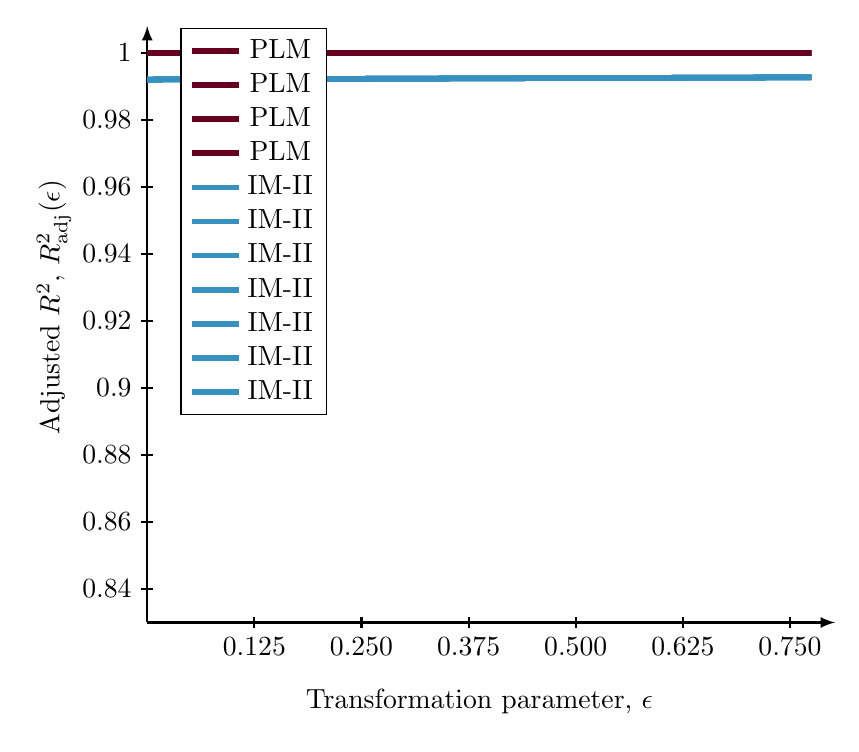
\begin{tikzpicture}
  % The axis of the plot
\begin{axis}[
    %title={Model: $\dv{y}{t}=\frac{2y}{t}$ with solution $y(t)=C_1t^2$\\Symmetry: $\Gamma_{\epsilon}=(t,y)\mapsto\left(\exp\left(\epsilon\right)t,\exp\left(-\epsilon\right)y\right)$},
    title style = {align=left},
    xlabel={Transformation parameter, $\epsilon$},
    ylabel={Adjusted $R^2$, $R^2_{\textrm{adj}}(\epsilon)$},
    %ylabel={Logarithm of Incidence, $\ln\left(R(t)\right)$},    
    % ylabel={Incidence, $R(t)$},
    x label style={at={(axis description cs:0.5,-0.1)},anchor=north},
    y label style={at={(axis description cs:-0.1,0.55)},rotate=90,anchor=south},    
    % xmin=-27, xmax=5,
    xmin=0, xmax=0.775,
    ymin = 0.83, ymax = 1.001,
    xtick={0,0.125,0.25,0.375,...,0.75},    
    %ymin=-14.5, ymax=1.5,
    %xtick={-30,-27,...,9},
    %ytick={1,0,-2,-4,-6,-8,-10,-12,-14},
    legend style={at={(axis description cs:0.05,0.7)},anchor=west},    
    %legend pos=north west,
    %ymajorgrids=true,
    grid style=dashed,
    x tick label style={
        /pgf/number format/.cd,
        fixed,
        fixed zerofill,
        precision=3,
        /tikz/.cd
    }
]    
]
% Plot the data
\addplot[
color=pow_1,line width=2pt,
]
coordinates {%
(0.0,1.0)
(0.10101010101010101,1.000000000000051)
(0.20202020202020202,0.999999999998303)
(0.30303030303030304,1.0000000000001539)
(0.40404040404040403,0.9999999999983028)
(0.5050505050505051,1.0000000000002565)
(0.6060606060606061,1.000000000000307)
(0.7070707070707071,0.999999999998303)
(0.8080808080808081,1.0000000000004097)
(0.9090909090909091,1.0000000000004612)
(1.0101010101010102,0.9999999999983027)
(1.1111111111111112,1.0000000000005638)
(1.2121212121212122,0.9999999999983029)
(1.3131313131313131,0.9999999999983028)
(1.4141414141414141,0.9999999999983028)
(1.5151515151515151,1.0000000000007685)
(1.6161616161616161,0.9999999999983029)
(1.7171717171717171,1.000000000000871)
(1.8181818181818181,0.9999999999983028)
(1.9191919191919191,1.0000000000009743)
(2.0202020202020203,1.0000000000010254)
(2.121212121212121,1.0000000000010765)
(2.2222222222222223,1.000000000001128)
(2.323232323232323,1.0000000000011795)
(2.4242424242424243,0.9999999999983029)
(2.525252525252525,0.9999999999983028)
(2.6262626262626263,1.0000000000013323)
(2.727272727272727,0.9999999999983029)
(2.8282828282828283,0.9999999999983028)
(2.929292929292929,0.9999999999983029)
(3.0303030303030303,0.9999999999983029)
(3.131313131313131,1.0000000000015896)
(3.2323232323232323,0.9999999999983029)
(3.3333333333333335,0.9999999999983028)
(3.4343434343434343,0.999999999998303)
(3.5353535353535355,1.0000000000017943)
(3.6363636363636362,1.0000000000018454)
(3.7373737373737375,1.0000000000018974)
(3.8383838383838382,1.0000000000019478)
(3.9393939393939394,1.0000000000019993)
(4.040404040404041,1.0000000000020506)
(4.141414141414141,0.9999999999983028)
(4.242424242424242,0.9999999999983029)
(4.343434343434343,0.9999999999983028)
(4.444444444444445,1.0000000000022569)
(4.545454545454545,1.0000000000023075)
(4.646464646464646,0.9999999999983028)
(4.747474747474747,0.9999999999983029)
(4.848484848484849,1.0000000000024623)
(4.94949494949495,1.000000000002512)
(5.05050505050505,0.999999999998303)
(5.151515151515151,1.0000000000026144)
(5.252525252525253,1.0000000000026665)
(5.353535353535354,1.000000000002718)
(5.454545454545454,0.9999999999983027)
(5.555555555555555,1.0000000000028204)
(5.656565656565657,1.0000000000028708)
(5.757575757575758,1.0000000000029228)
(5.858585858585858,0.9999999999983029)
(5.959595959595959,0.9999999999983027)
(6.0606060606060606,1.0000000000030764)
(6.161616161616162,1.0000000000031275)
(6.262626262626262,1.0000000000031783)
(6.363636363636363,1.0000000000032296)
(6.4646464646464645,1.000000000003282)
(6.565656565656566,1.0000000000033318)
(6.666666666666667,1.000000000003384)
(6.767676767676767,1.0000000000034348)
(6.8686868686868685,1.0000000000034859)
(6.96969696969697,0.9999999999983027)
(7.070707070707071,1.00000000000359)
(7.171717171717171,1.000000000003641)
(7.2727272727272725,1.0000000000036908)
(7.373737373737374,0.999999999998303)
(7.474747474747475,1.000000000003795)
(7.575757575757575,0.9999999999983027)
(7.6767676767676765,1.0000000000038956)
(7.777777777777778,0.9999999999983027)
(7.878787878787879,0.9999999999983029)
(7.979797979797979,1.0000000000040505)
(8.080808080808081,1.0000000000041016)
(8.181818181818182,1.0000000000041547)
(8.282828282828282,0.9999999999983031)
(8.383838383838384,0.9999999999983029)
(8.484848484848484,1.0000000000043072)
(8.585858585858587,1.0000000000043585)
(8.686868686868687,0.999999999998303)
(8.787878787878787,1.0000000000044604)
(8.88888888888889,0.9999999999983029)
(8.98989898989899,1.0000000000045648)
(9.09090909090909,1.000000000004614)
(9.191919191919192,1.0000000000046658)
(9.292929292929292,1.000000000004718)
(9.393939393939394,1.000000000004769)
(9.494949494949495,0.9999999999983032)
(9.595959595959595,1.0000000000048725)
(9.696969696969697,1.0000000000049225)
(9.797979797979798,1.0000000000049725)
(9.8989898989899,1.0000000000050229)
(10.0,1.0000000000050784)
};
\addlegendentry{PLM}
\addplot[
color=pow_1,line width=2pt,
]
coordinates {%
(0.0,1.0)
(0.10101010101010101,1.000000000000051)
(0.20202020202020202,0.999999999998303)
(0.30303030303030304,1.0000000000001539)
(0.40404040404040403,0.9999999999983028)
(0.5050505050505051,1.0000000000002565)
(0.6060606060606061,1.000000000000307)
(0.7070707070707071,0.999999999998303)
(0.8080808080808081,1.0000000000004097)
(0.9090909090909091,1.0000000000004612)
(1.0101010101010102,0.9999999999983027)
(1.1111111111111112,1.0000000000005638)
(1.2121212121212122,0.9999999999983029)
(1.3131313131313131,0.9999999999983028)
(1.4141414141414141,0.9999999999983028)
(1.5151515151515151,1.0000000000007685)
(1.6161616161616161,0.9999999999983029)
(1.7171717171717171,1.000000000000871)
(1.8181818181818181,0.9999999999983028)
(1.9191919191919191,1.0000000000009743)
(2.0202020202020203,1.0000000000010254)
(2.121212121212121,1.0000000000010765)
(2.2222222222222223,1.000000000001128)
(2.323232323232323,1.0000000000011795)
(2.4242424242424243,0.9999999999983029)
(2.525252525252525,0.9999999999983028)
(2.6262626262626263,1.0000000000013323)
(2.727272727272727,0.9999999999983029)
(2.8282828282828283,0.9999999999983028)
(2.929292929292929,0.9999999999983029)
(3.0303030303030303,0.9999999999983029)
(3.131313131313131,1.0000000000015896)
(3.2323232323232323,0.9999999999983029)
(3.3333333333333335,0.9999999999983028)
(3.4343434343434343,0.999999999998303)
(3.5353535353535355,1.0000000000017943)
(3.6363636363636362,1.0000000000018454)
(3.7373737373737375,1.0000000000018974)
(3.8383838383838382,1.0000000000019478)
(3.9393939393939394,1.0000000000019993)
(4.040404040404041,1.0000000000020506)
(4.141414141414141,0.9999999999983028)
(4.242424242424242,0.9999999999983029)
(4.343434343434343,0.9999999999983028)
(4.444444444444445,1.0000000000022569)
(4.545454545454545,1.0000000000023075)
(4.646464646464646,0.9999999999983028)
(4.747474747474747,0.9999999999983029)
(4.848484848484849,1.0000000000024623)
(4.94949494949495,1.000000000002512)
(5.05050505050505,0.999999999998303)
(5.151515151515151,1.0000000000026144)
(5.252525252525253,1.0000000000026665)
(5.353535353535354,1.000000000002718)
(5.454545454545454,0.9999999999983027)
(5.555555555555555,1.0000000000028204)
(5.656565656565657,1.0000000000028708)
(5.757575757575758,1.0000000000029228)
(5.858585858585858,0.9999999999983029)
(5.959595959595959,0.9999999999983027)
(6.0606060606060606,1.0000000000030764)
(6.161616161616162,1.0000000000031275)
(6.262626262626262,1.0000000000031783)
(6.363636363636363,1.0000000000032296)
(6.4646464646464645,1.000000000003282)
(6.565656565656566,1.0000000000033318)
(6.666666666666667,1.000000000003384)
(6.767676767676767,1.0000000000034348)
(6.8686868686868685,1.0000000000034859)
(6.96969696969697,0.9999999999983027)
(7.070707070707071,1.00000000000359)
(7.171717171717171,1.000000000003641)
(7.2727272727272725,1.0000000000036908)
(7.373737373737374,0.999999999998303)
(7.474747474747475,1.000000000003795)
(7.575757575757575,0.9999999999983027)
(7.6767676767676765,1.0000000000038956)
(7.777777777777778,0.9999999999983027)
(7.878787878787879,0.9999999999983029)
(7.979797979797979,1.0000000000040505)
(8.080808080808081,1.0000000000041016)
(8.181818181818182,1.0000000000041547)
(8.282828282828282,0.9999999999983031)
(8.383838383838384,0.9999999999983029)
(8.484848484848484,1.0000000000043072)
(8.585858585858587,1.0000000000043585)
(8.686868686868687,0.999999999998303)
(8.787878787878787,1.0000000000044604)
(8.88888888888889,0.9999999999983029)
(8.98989898989899,1.0000000000045648)
(9.09090909090909,1.000000000004614)
(9.191919191919192,1.0000000000046658)
(9.292929292929292,1.000000000004718)
(9.393939393939394,1.000000000004769)
(9.494949494949495,0.9999999999983032)
(9.595959595959595,1.0000000000048725)
(9.696969696969697,1.0000000000049225)
(9.797979797979798,1.0000000000049725)
(9.8989898989899,1.0000000000050229)
(10.0,1.0000000000050784)
};
\addlegendentry{PLM}
\addplot[
color=pow_1,line width=2pt,
]
coordinates {%
(0.0,1.0)
(0.10101010101010101,1.000000000000051)
(0.20202020202020202,0.999999999998303)
(0.30303030303030304,1.0000000000001539)
(0.40404040404040403,0.9999999999983028)
(0.5050505050505051,1.0000000000002565)
(0.6060606060606061,1.000000000000307)
(0.7070707070707071,0.999999999998303)
(0.8080808080808081,1.0000000000004097)
(0.9090909090909091,1.0000000000004612)
(1.0101010101010102,0.9999999999983027)
(1.1111111111111112,1.0000000000005638)
(1.2121212121212122,0.9999999999983029)
(1.3131313131313131,0.9999999999983028)
(1.4141414141414141,0.9999999999983028)
(1.5151515151515151,1.0000000000007685)
(1.6161616161616161,0.9999999999983029)
(1.7171717171717171,1.000000000000871)
(1.8181818181818181,0.9999999999983028)
(1.9191919191919191,1.0000000000009743)
(2.0202020202020203,1.0000000000010254)
(2.121212121212121,1.0000000000010765)
(2.2222222222222223,1.000000000001128)
(2.323232323232323,1.0000000000011795)
(2.4242424242424243,0.9999999999983029)
(2.525252525252525,0.9999999999983028)
(2.6262626262626263,1.0000000000013323)
(2.727272727272727,0.9999999999983029)
(2.8282828282828283,0.9999999999983028)
(2.929292929292929,0.9999999999983029)
(3.0303030303030303,0.9999999999983029)
(3.131313131313131,1.0000000000015896)
(3.2323232323232323,0.9999999999983029)
(3.3333333333333335,0.9999999999983028)
(3.4343434343434343,0.999999999998303)
(3.5353535353535355,1.0000000000017943)
(3.6363636363636362,1.0000000000018454)
(3.7373737373737375,1.0000000000018974)
(3.8383838383838382,1.0000000000019478)
(3.9393939393939394,1.0000000000019993)
(4.040404040404041,1.0000000000020506)
(4.141414141414141,0.9999999999983028)
(4.242424242424242,0.9999999999983029)
(4.343434343434343,0.9999999999983028)
(4.444444444444445,1.0000000000022569)
(4.545454545454545,1.0000000000023075)
(4.646464646464646,0.9999999999983028)
(4.747474747474747,0.9999999999983029)
(4.848484848484849,1.0000000000024623)
(4.94949494949495,1.000000000002512)
(5.05050505050505,0.999999999998303)
(5.151515151515151,1.0000000000026144)
(5.252525252525253,1.0000000000026665)
(5.353535353535354,1.000000000002718)
(5.454545454545454,0.9999999999983027)
(5.555555555555555,1.0000000000028204)
(5.656565656565657,1.0000000000028708)
(5.757575757575758,1.0000000000029228)
(5.858585858585858,0.9999999999983029)
(5.959595959595959,0.9999999999983027)
(6.0606060606060606,1.0000000000030764)
(6.161616161616162,1.0000000000031275)
(6.262626262626262,1.0000000000031783)
(6.363636363636363,1.0000000000032296)
(6.4646464646464645,1.000000000003282)
(6.565656565656566,1.0000000000033318)
(6.666666666666667,1.000000000003384)
(6.767676767676767,1.0000000000034348)
(6.8686868686868685,1.0000000000034859)
(6.96969696969697,0.9999999999983027)
(7.070707070707071,1.00000000000359)
(7.171717171717171,1.000000000003641)
(7.2727272727272725,1.0000000000036908)
(7.373737373737374,0.999999999998303)
(7.474747474747475,1.000000000003795)
(7.575757575757575,0.9999999999983027)
(7.6767676767676765,1.0000000000038956)
(7.777777777777778,0.9999999999983027)
(7.878787878787879,0.9999999999983029)
(7.979797979797979,1.0000000000040505)
(8.080808080808081,1.0000000000041016)
(8.181818181818182,1.0000000000041547)
(8.282828282828282,0.9999999999983031)
(8.383838383838384,0.9999999999983029)
(8.484848484848484,1.0000000000043072)
(8.585858585858587,1.0000000000043585)
(8.686868686868687,0.999999999998303)
(8.787878787878787,1.0000000000044604)
(8.88888888888889,0.9999999999983029)
(8.98989898989899,1.0000000000045648)
(9.09090909090909,1.000000000004614)
(9.191919191919192,1.0000000000046658)
(9.292929292929292,1.000000000004718)
(9.393939393939394,1.000000000004769)
(9.494949494949495,0.9999999999983032)
(9.595959595959595,1.0000000000048725)
(9.696969696969697,1.0000000000049225)
(9.797979797979798,1.0000000000049725)
(9.8989898989899,1.0000000000050229)
(10.0,1.0000000000050784)
};
\addlegendentry{PLM}
\addplot[
color=pow_1,line width=2pt,
]
coordinates {%
(0.0,1.0)
(0.10101010101010101,1.000000000000051)
(0.20202020202020202,0.999999999998303)
(0.30303030303030304,1.0000000000001539)
(0.40404040404040403,0.9999999999983028)
(0.5050505050505051,1.0000000000002565)
(0.6060606060606061,1.000000000000307)
(0.7070707070707071,0.999999999998303)
(0.8080808080808081,1.0000000000004097)
(0.9090909090909091,1.0000000000004612)
(1.0101010101010102,0.9999999999983027)
(1.1111111111111112,1.0000000000005638)
(1.2121212121212122,0.9999999999983029)
(1.3131313131313131,0.9999999999983028)
(1.4141414141414141,0.9999999999983028)
(1.5151515151515151,1.0000000000007685)
(1.6161616161616161,0.9999999999983029)
(1.7171717171717171,1.000000000000871)
(1.8181818181818181,0.9999999999983028)
(1.9191919191919191,1.0000000000009743)
(2.0202020202020203,1.0000000000010254)
(2.121212121212121,1.0000000000010765)
(2.2222222222222223,1.000000000001128)
(2.323232323232323,1.0000000000011795)
(2.4242424242424243,0.9999999999983029)
(2.525252525252525,0.9999999999983028)
(2.6262626262626263,1.0000000000013323)
(2.727272727272727,0.9999999999983029)
(2.8282828282828283,0.9999999999983028)
(2.929292929292929,0.9999999999983029)
(3.0303030303030303,0.9999999999983029)
(3.131313131313131,1.0000000000015896)
(3.2323232323232323,0.9999999999983029)
(3.3333333333333335,0.9999999999983028)
(3.4343434343434343,0.999999999998303)
(3.5353535353535355,1.0000000000017943)
(3.6363636363636362,1.0000000000018454)
(3.7373737373737375,1.0000000000018974)
(3.8383838383838382,1.0000000000019478)
(3.9393939393939394,1.0000000000019993)
(4.040404040404041,1.0000000000020506)
(4.141414141414141,0.9999999999983028)
(4.242424242424242,0.9999999999983029)
(4.343434343434343,0.9999999999983028)
(4.444444444444445,1.0000000000022569)
(4.545454545454545,1.0000000000023075)
(4.646464646464646,0.9999999999983028)
(4.747474747474747,0.9999999999983029)
(4.848484848484849,1.0000000000024623)
(4.94949494949495,1.000000000002512)
(5.05050505050505,0.999999999998303)
(5.151515151515151,1.0000000000026144)
(5.252525252525253,1.0000000000026665)
(5.353535353535354,1.000000000002718)
(5.454545454545454,0.9999999999983027)
(5.555555555555555,1.0000000000028204)
(5.656565656565657,1.0000000000028708)
(5.757575757575758,1.0000000000029228)
(5.858585858585858,0.9999999999983029)
(5.959595959595959,0.9999999999983027)
(6.0606060606060606,1.0000000000030764)
(6.161616161616162,1.0000000000031275)
(6.262626262626262,1.0000000000031783)
(6.363636363636363,1.0000000000032296)
(6.4646464646464645,1.000000000003282)
(6.565656565656566,1.0000000000033318)
(6.666666666666667,1.000000000003384)
(6.767676767676767,1.0000000000034348)
(6.8686868686868685,1.0000000000034859)
(6.96969696969697,0.9999999999983027)
(7.070707070707071,1.00000000000359)
(7.171717171717171,1.000000000003641)
(7.2727272727272725,1.0000000000036908)
(7.373737373737374,0.999999999998303)
(7.474747474747475,1.000000000003795)
(7.575757575757575,0.9999999999983027)
(7.6767676767676765,1.0000000000038956)
(7.777777777777778,0.9999999999983027)
(7.878787878787879,0.9999999999983029)
(7.979797979797979,1.0000000000040505)
(8.080808080808081,1.0000000000041016)
(8.181818181818182,1.0000000000041547)
(8.282828282828282,0.9999999999983031)
(8.383838383838384,0.9999999999983029)
(8.484848484848484,1.0000000000043072)
(8.585858585858587,1.0000000000043585)
(8.686868686868687,0.999999999998303)
(8.787878787878787,1.0000000000044604)
(8.88888888888889,0.9999999999983029)
(8.98989898989899,1.0000000000045648)
(9.09090909090909,1.000000000004614)
(9.191919191919192,1.0000000000046658)
(9.292929292929292,1.000000000004718)
(9.393939393939394,1.000000000004769)
(9.494949494949495,0.9999999999983032)
(9.595959595959595,1.0000000000048725)
(9.696969696969697,1.0000000000049225)
(9.797979797979798,1.0000000000049725)
(9.8989898989899,1.0000000000050229)
(10.0,1.0000000000050784)
};
\addlegendentry{PLM}

% Plot the model
\addplot[
color=mixed_2,line width=2pt,
]
coordinates {%
(0.0,0.9920681275409042)
(0.10101010101010101,0.9921614378587185)
(0.20202020202020202,0.9922524571179404)
(0.30303030303030304,0.9923411225750451)
(0.40404040404040403,0.9924273694312656)
(0.5050505050505051,0.9925111307470728)
(0.6060606060606061,0.9925923373522489)
(0.7070707070707071,0.9926709177512789)
(0.8080808080808081,0.9927467980237661)
(0.9090909090909091,0.9928199017195577)
(1.0101010101010102,0.9928901497482401)
(1.1111111111111112,0.9929574602626406)
(1.2121212121212122,0.993021748535942)
(1.3131313131313131,0.9930829268319884)
(1.4141414141414141,0.9931409042683254)
(1.5151515151515151,0.9931955866714859)
(1.6161616161616161,0.993246876423987)
(1.7171717171717171,0.9932946723024673)
(1.8181818181818181,0.9933388693063415)
(1.9191919191919191,0.9933793584763044)
(2.0202020202020203,0.993416026701952)
(2.121212121212121,0.9934487565177325)
(2.2222222222222223,0.9934774258863688)
(2.323232323232323,0.9935019079688225)
(2.4242424242424243,0.9935220708797817)
(2.525252525252525,0.9935377774275728)
(2.6262626262626263,0.993548884837289)
(2.727272727272727,0.9935552444558251)
(2.8282828282828283,0.993556701437378)
(2.929292929292929,0.9935530944078471)
(3.0303030303030303,0.9935442551064124)
(3.131313131313131,0.9935300080024019)
(3.2323232323232323,0.9935101698853807)
(3.3333333333333335,0.9934845494261807)
(3.4343434343434343,0.9934529467063677)
(3.5353535353535355,0.993415152713378)
(3.6363636363636362,0.9933709487982765)
(3.7373737373737375,0.9933201060927607)
(3.8383838383838382,0.9932623848816786)
(3.9393939393939394,0.9931975339269151)
(4.040404040404041,0.9931252897380471)
(4.141414141414141,0.9930453757846521)
(4.242424242424242,0.9929575016445609)
(4.343434343434343,0.99286136208169)
(4.444444444444445,0.992756636046329)
(4.545454545454545,0.9926429855899029)
(4.646464646464646,0.9925200546852463)
(4.747474747474747,0.9923874679423099)
(4.848484848484849,0.9922448292079341)
(4.94949494949495,0.9920917200368463)
(5.05050505050505,0.9919276980193459)
(5.151515151515151,0.9917522949491694)
(5.252525252525253,0.9915650148127608)
(5.353535353535354,0.9913653315785309)
(5.454545454545454,0.9911526867616066)
(5.555555555555555,0.9909264867359864)
(5.656565656565657,0.9906860997617926)
(5.757575757575758,0.9904308526903618)
(5.858585858585858,0.9901600273040526)
(5.959595959595959,0.9898728562407261)
(6.0606060606060606,0.9895685184445934)
(6.161616161616162,0.9892461340752863)
(6.262626262626262,0.9889047587951851)
(6.363636363636363,0.9885433773408155)
(6.4646464646464645,0.9881608962669033)
(6.565656565656566,0.9877561357307344)
(6.666666666666667,0.9873278201588752)
(6.767676767676767,0.9868745676068427)
(6.8686868686868685,0.9863948775834264)
(6.96969696969697,0.9858871170630049)
(7.070707070707071,0.985349504348661)
(7.171717171717171,0.9847800903726148)
(7.2727272727272725,0.9841767369236564)
(7.373737373737374,0.9835370911673763)
(7.474747474747475,0.9828585556652083)
(7.575757575757575,0.9821382528903685)
(7.6767676767676765,0.9813729829656376)
(7.777777777777778,0.9805591729854569)
(7.878787878787879,0.9796928157984839)
(7.979797979797979,0.9787693954664941)
(8.080808080808081,0.9777837957075278)
(8.181818181818182,0.9767301863649741)
(8.282828282828282,0.9756018811514188)
(8.383838383838384,0.9743911573347532)
(8.484848484848484,0.9730890242485605)
(8.585858585858587,0.971684921843413)
(8.686868686868687,0.9701663218230534)
(8.787878787878787,0.9685181902932143)
(8.88888888888889,0.9667222488558476)
(8.98989898989899,0.9647559343856933)
(9.09090909090909,0.9625908941984097)
(9.191919191919192,0.9601907385390367)
(9.292929292929292,0.9575075543042407)
(9.393939393939394,0.9544762444900531)
(9.494949494949495,0.9510048063272181)
(9.595959595959595,0.9469564096175731)
(9.696969696969697,0.9421131727370925)
(9.797979797979798,0.9360931780165072)
(9.8989898989899,0.9281223973816773)
(10.0,0.9161907031749841)
};
\addlegendentry{IM-II}
\addplot[
color=mixed_2,line width=2pt,
]
coordinates {%
(0.0,0.9920681275409042)
(0.10101010101010101,0.9921614378587185)
(0.20202020202020202,0.9922524571179404)
(0.30303030303030304,0.9923411225750451)
(0.40404040404040403,0.9924273694312656)
(0.5050505050505051,0.9925111307470728)
(0.6060606060606061,0.9925923373522489)
(0.7070707070707071,0.9926709177512789)
(0.8080808080808081,0.9927467980237661)
(0.9090909090909091,0.9928199017195577)
(1.0101010101010102,0.9928901497482401)
(1.1111111111111112,0.9929574602626406)
(1.2121212121212122,0.993021748535942)
(1.3131313131313131,0.9930829268319884)
(1.4141414141414141,0.9931409042683254)
(1.5151515151515151,0.9931955866714859)
(1.6161616161616161,0.993246876423987)
(1.7171717171717171,0.9932946723024673)
(1.8181818181818181,0.9933388693063415)
(1.9191919191919191,0.9933793584763044)
(2.0202020202020203,0.993416026701952)
(2.121212121212121,0.9934487565177325)
(2.2222222222222223,0.9934774258863688)
(2.323232323232323,0.9935019079688225)
(2.4242424242424243,0.9935220708797817)
(2.525252525252525,0.9935377774275728)
(2.6262626262626263,0.993548884837289)
(2.727272727272727,0.9935552444558251)
(2.8282828282828283,0.993556701437378)
(2.929292929292929,0.9935530944078471)
(3.0303030303030303,0.9935442551064124)
(3.131313131313131,0.9935300080024019)
(3.2323232323232323,0.9935101698853807)
(3.3333333333333335,0.9934845494261807)
(3.4343434343434343,0.9934529467063677)
(3.5353535353535355,0.993415152713378)
(3.6363636363636362,0.9933709487982765)
(3.7373737373737375,0.9933201060927607)
(3.8383838383838382,0.9932623848816786)
(3.9393939393939394,0.9931975339269151)
(4.040404040404041,0.9931252897380471)
(4.141414141414141,0.9930453757846521)
(4.242424242424242,0.9929575016445609)
(4.343434343434343,0.99286136208169)
(4.444444444444445,0.992756636046329)
(4.545454545454545,0.9926429855899029)
(4.646464646464646,0.9925200546852463)
(4.747474747474747,0.9923874679423099)
(4.848484848484849,0.9922448292079341)
(4.94949494949495,0.9920917200368463)
(5.05050505050505,0.9919276980193459)
(5.151515151515151,0.9917522949491694)
(5.252525252525253,0.9915650148127608)
(5.353535353535354,0.9913653315785309)
(5.454545454545454,0.9911526867616066)
(5.555555555555555,0.9909264867359864)
(5.656565656565657,0.9906860997617926)
(5.757575757575758,0.9904308526903618)
(5.858585858585858,0.9901600273040526)
(5.959595959595959,0.9898728562407261)
(6.0606060606060606,0.9895685184445934)
(6.161616161616162,0.9892461340752863)
(6.262626262626262,0.9889047587951851)
(6.363636363636363,0.9885433773408155)
(6.4646464646464645,0.9881608962669033)
(6.565656565656566,0.9877561357307344)
(6.666666666666667,0.9873278201588752)
(6.767676767676767,0.9868745676068427)
(6.8686868686868685,0.9863948775834264)
(6.96969696969697,0.9858871170630049)
(7.070707070707071,0.985349504348661)
(7.171717171717171,0.9847800903726148)
(7.2727272727272725,0.9841767369236564)
(7.373737373737374,0.9835370911673763)
(7.474747474747475,0.9828585556652083)
(7.575757575757575,0.9821382528903685)
(7.6767676767676765,0.9813729829656376)
(7.777777777777778,0.9805591729854569)
(7.878787878787879,0.9796928157984839)
(7.979797979797979,0.9787693954664941)
(8.080808080808081,0.9777837957075278)
(8.181818181818182,0.9767301863649741)
(8.282828282828282,0.9756018811514188)
(8.383838383838384,0.9743911573347532)
(8.484848484848484,0.9730890242485605)
(8.585858585858587,0.971684921843413)
(8.686868686868687,0.9701663218230534)
(8.787878787878787,0.9685181902932143)
(8.88888888888889,0.9667222488558476)
(8.98989898989899,0.9647559343856933)
(9.09090909090909,0.9625908941984097)
(9.191919191919192,0.9601907385390367)
(9.292929292929292,0.9575075543042407)
(9.393939393939394,0.9544762444900531)
(9.494949494949495,0.9510048063272181)
(9.595959595959595,0.9469564096175731)
(9.696969696969697,0.9421131727370925)
(9.797979797979798,0.9360931780165072)
(9.8989898989899,0.9281223973816773)
(10.0,0.9161907031749841)
};
\addlegendentry{IM-II}
\addplot[
color=mixed_2,line width=2pt,
]
coordinates {%
(0.0,0.9920681275409042)
(0.10101010101010101,0.9921614378587185)
(0.20202020202020202,0.9922524571179404)
(0.30303030303030304,0.9923411225750451)
(0.40404040404040403,0.9924273694312656)
(0.5050505050505051,0.9925111307470728)
(0.6060606060606061,0.9925923373522489)
(0.7070707070707071,0.9926709177512789)
(0.8080808080808081,0.9927467980237661)
(0.9090909090909091,0.9928199017195577)
(1.0101010101010102,0.9928901497482401)
(1.1111111111111112,0.9929574602626406)
(1.2121212121212122,0.993021748535942)
(1.3131313131313131,0.9930829268319884)
(1.4141414141414141,0.9931409042683254)
(1.5151515151515151,0.9931955866714859)
(1.6161616161616161,0.993246876423987)
(1.7171717171717171,0.9932946723024673)
(1.8181818181818181,0.9933388693063415)
(1.9191919191919191,0.9933793584763044)
(2.0202020202020203,0.993416026701952)
(2.121212121212121,0.9934487565177325)
(2.2222222222222223,0.9934774258863688)
(2.323232323232323,0.9935019079688225)
(2.4242424242424243,0.9935220708797817)
(2.525252525252525,0.9935377774275728)
(2.6262626262626263,0.993548884837289)
(2.727272727272727,0.9935552444558251)
(2.8282828282828283,0.993556701437378)
(2.929292929292929,0.9935530944078471)
(3.0303030303030303,0.9935442551064124)
(3.131313131313131,0.9935300080024019)
(3.2323232323232323,0.9935101698853807)
(3.3333333333333335,0.9934845494261807)
(3.4343434343434343,0.9934529467063677)
(3.5353535353535355,0.993415152713378)
(3.6363636363636362,0.9933709487982765)
(3.7373737373737375,0.9933201060927607)
(3.8383838383838382,0.9932623848816786)
(3.9393939393939394,0.9931975339269151)
(4.040404040404041,0.9931252897380471)
(4.141414141414141,0.9930453757846521)
(4.242424242424242,0.9929575016445609)
(4.343434343434343,0.99286136208169)
(4.444444444444445,0.992756636046329)
(4.545454545454545,0.9926429855899029)
(4.646464646464646,0.9925200546852463)
(4.747474747474747,0.9923874679423099)
(4.848484848484849,0.9922448292079341)
(4.94949494949495,0.9920917200368463)
(5.05050505050505,0.9919276980193459)
(5.151515151515151,0.9917522949491694)
(5.252525252525253,0.9915650148127608)
(5.353535353535354,0.9913653315785309)
(5.454545454545454,0.9911526867616066)
(5.555555555555555,0.9909264867359864)
(5.656565656565657,0.9906860997617926)
(5.757575757575758,0.9904308526903618)
(5.858585858585858,0.9901600273040526)
(5.959595959595959,0.9898728562407261)
(6.0606060606060606,0.9895685184445934)
(6.161616161616162,0.9892461340752863)
(6.262626262626262,0.9889047587951851)
(6.363636363636363,0.9885433773408155)
(6.4646464646464645,0.9881608962669033)
(6.565656565656566,0.9877561357307344)
(6.666666666666667,0.9873278201588752)
(6.767676767676767,0.9868745676068427)
(6.8686868686868685,0.9863948775834264)
(6.96969696969697,0.9858871170630049)
(7.070707070707071,0.985349504348661)
(7.171717171717171,0.9847800903726148)
(7.2727272727272725,0.9841767369236564)
(7.373737373737374,0.9835370911673763)
(7.474747474747475,0.9828585556652083)
(7.575757575757575,0.9821382528903685)
(7.6767676767676765,0.9813729829656376)
(7.777777777777778,0.9805591729854569)
(7.878787878787879,0.9796928157984839)
(7.979797979797979,0.9787693954664941)
(8.080808080808081,0.9777837957075278)
(8.181818181818182,0.9767301863649741)
(8.282828282828282,0.9756018811514188)
(8.383838383838384,0.9743911573347532)
(8.484848484848484,0.9730890242485605)
(8.585858585858587,0.971684921843413)
(8.686868686868687,0.9701663218230534)
(8.787878787878787,0.9685181902932143)
(8.88888888888889,0.9667222488558476)
(8.98989898989899,0.9647559343856933)
(9.09090909090909,0.9625908941984097)
(9.191919191919192,0.9601907385390367)
(9.292929292929292,0.9575075543042407)
(9.393939393939394,0.9544762444900531)
(9.494949494949495,0.9510048063272181)
(9.595959595959595,0.9469564096175731)
(9.696969696969697,0.9421131727370925)
(9.797979797979798,0.9360931780165072)
(9.8989898989899,0.9281223973816773)
(10.0,0.9161907031749841)
};
\addlegendentry{IM-II}
\addplot[
color=mixed_2,line width=2pt,
]
coordinates {%
(0.0,0.9920681275409042)
(0.10101010101010101,0.9921614378587185)
(0.20202020202020202,0.9922524571179404)
(0.30303030303030304,0.9923411225750451)
(0.40404040404040403,0.9924273694312656)
(0.5050505050505051,0.9925111307470728)
(0.6060606060606061,0.9925923373522489)
(0.7070707070707071,0.9926709177512789)
(0.8080808080808081,0.9927467980237661)
(0.9090909090909091,0.9928199017195577)
(1.0101010101010102,0.9928901497482401)
(1.1111111111111112,0.9929574602626406)
(1.2121212121212122,0.993021748535942)
(1.3131313131313131,0.9930829268319884)
(1.4141414141414141,0.9931409042683254)
(1.5151515151515151,0.9931955866714859)
(1.6161616161616161,0.993246876423987)
(1.7171717171717171,0.9932946723024673)
(1.8181818181818181,0.9933388693063415)
(1.9191919191919191,0.9933793584763044)
(2.0202020202020203,0.993416026701952)
(2.121212121212121,0.9934487565177325)
(2.2222222222222223,0.9934774258863688)
(2.323232323232323,0.9935019079688225)
(2.4242424242424243,0.9935220708797817)
(2.525252525252525,0.9935377774275728)
(2.6262626262626263,0.993548884837289)
(2.727272727272727,0.9935552444558251)
(2.8282828282828283,0.993556701437378)
(2.929292929292929,0.9935530944078471)
(3.0303030303030303,0.9935442551064124)
(3.131313131313131,0.9935300080024019)
(3.2323232323232323,0.9935101698853807)
(3.3333333333333335,0.9934845494261807)
(3.4343434343434343,0.9934529467063677)
(3.5353535353535355,0.993415152713378)
(3.6363636363636362,0.9933709487982765)
(3.7373737373737375,0.9933201060927607)
(3.8383838383838382,0.9932623848816786)
(3.9393939393939394,0.9931975339269151)
(4.040404040404041,0.9931252897380471)
(4.141414141414141,0.9930453757846521)
(4.242424242424242,0.9929575016445609)
(4.343434343434343,0.99286136208169)
(4.444444444444445,0.992756636046329)
(4.545454545454545,0.9926429855899029)
(4.646464646464646,0.9925200546852463)
(4.747474747474747,0.9923874679423099)
(4.848484848484849,0.9922448292079341)
(4.94949494949495,0.9920917200368463)
(5.05050505050505,0.9919276980193459)
(5.151515151515151,0.9917522949491694)
(5.252525252525253,0.9915650148127608)
(5.353535353535354,0.9913653315785309)
(5.454545454545454,0.9911526867616066)
(5.555555555555555,0.9909264867359864)
(5.656565656565657,0.9906860997617926)
(5.757575757575758,0.9904308526903618)
(5.858585858585858,0.9901600273040526)
(5.959595959595959,0.9898728562407261)
(6.0606060606060606,0.9895685184445934)
(6.161616161616162,0.9892461340752863)
(6.262626262626262,0.9889047587951851)
(6.363636363636363,0.9885433773408155)
(6.4646464646464645,0.9881608962669033)
(6.565656565656566,0.9877561357307344)
(6.666666666666667,0.9873278201588752)
(6.767676767676767,0.9868745676068427)
(6.8686868686868685,0.9863948775834264)
(6.96969696969697,0.9858871170630049)
(7.070707070707071,0.985349504348661)
(7.171717171717171,0.9847800903726148)
(7.2727272727272725,0.9841767369236564)
(7.373737373737374,0.9835370911673763)
(7.474747474747475,0.9828585556652083)
(7.575757575757575,0.9821382528903685)
(7.6767676767676765,0.9813729829656376)
(7.777777777777778,0.9805591729854569)
(7.878787878787879,0.9796928157984839)
(7.979797979797979,0.9787693954664941)
(8.080808080808081,0.9777837957075278)
(8.181818181818182,0.9767301863649741)
(8.282828282828282,0.9756018811514188)
(8.383838383838384,0.9743911573347532)
(8.484848484848484,0.9730890242485605)
(8.585858585858587,0.971684921843413)
(8.686868686868687,0.9701663218230534)
(8.787878787878787,0.9685181902932143)
(8.88888888888889,0.9667222488558476)
(8.98989898989899,0.9647559343856933)
(9.09090909090909,0.9625908941984097)
(9.191919191919192,0.9601907385390367)
(9.292929292929292,0.9575075543042407)
(9.393939393939394,0.9544762444900531)
(9.494949494949495,0.9510048063272181)
(9.595959595959595,0.9469564096175731)
(9.696969696969697,0.9421131727370925)
(9.797979797979798,0.9360931780165072)
(9.8989898989899,0.9281223973816773)
(10.0,0.9161907031749841)
};
\addlegendentry{IM-II}
\addplot[
color=mixed_2,line width=2pt,
]
coordinates {%
(0.0,0.9920681275409042)
(0.10101010101010101,0.9921614378587185)
(0.20202020202020202,0.9922524571179404)
(0.30303030303030304,0.9923411225750451)
(0.40404040404040403,0.9924273694312656)
(0.5050505050505051,0.9925111307470728)
(0.6060606060606061,0.9925923373522489)
(0.7070707070707071,0.9926709177512789)
(0.8080808080808081,0.9927467980237661)
(0.9090909090909091,0.9928199017195577)
(1.0101010101010102,0.9928901497482401)
(1.1111111111111112,0.9929574602626406)
(1.2121212121212122,0.993021748535942)
(1.3131313131313131,0.9930829268319884)
(1.4141414141414141,0.9931409042683254)
(1.5151515151515151,0.9931955866714859)
(1.6161616161616161,0.993246876423987)
(1.7171717171717171,0.9932946723024673)
(1.8181818181818181,0.9933388693063415)
(1.9191919191919191,0.9933793584763044)
(2.0202020202020203,0.993416026701952)
(2.121212121212121,0.9934487565177325)
(2.2222222222222223,0.9934774258863688)
(2.323232323232323,0.9935019079688225)
(2.4242424242424243,0.9935220708797817)
(2.525252525252525,0.9935377774275728)
(2.6262626262626263,0.993548884837289)
(2.727272727272727,0.9935552444558251)
(2.8282828282828283,0.993556701437378)
(2.929292929292929,0.9935530944078471)
(3.0303030303030303,0.9935442551064124)
(3.131313131313131,0.9935300080024019)
(3.2323232323232323,0.9935101698853807)
(3.3333333333333335,0.9934845494261807)
(3.4343434343434343,0.9934529467063677)
(3.5353535353535355,0.993415152713378)
(3.6363636363636362,0.9933709487982765)
(3.7373737373737375,0.9933201060927607)
(3.8383838383838382,0.9932623848816786)
(3.9393939393939394,0.9931975339269151)
(4.040404040404041,0.9931252897380471)
(4.141414141414141,0.9930453757846521)
(4.242424242424242,0.9929575016445609)
(4.343434343434343,0.99286136208169)
(4.444444444444445,0.992756636046329)
(4.545454545454545,0.9926429855899029)
(4.646464646464646,0.9925200546852463)
(4.747474747474747,0.9923874679423099)
(4.848484848484849,0.9922448292079341)
(4.94949494949495,0.9920917200368463)
(5.05050505050505,0.9919276980193459)
(5.151515151515151,0.9917522949491694)
(5.252525252525253,0.9915650148127608)
(5.353535353535354,0.9913653315785309)
(5.454545454545454,0.9911526867616066)
(5.555555555555555,0.9909264867359864)
(5.656565656565657,0.9906860997617926)
(5.757575757575758,0.9904308526903618)
(5.858585858585858,0.9901600273040526)
(5.959595959595959,0.9898728562407261)
(6.0606060606060606,0.9895685184445934)
(6.161616161616162,0.9892461340752863)
(6.262626262626262,0.9889047587951851)
(6.363636363636363,0.9885433773408155)
(6.4646464646464645,0.9881608962669033)
(6.565656565656566,0.9877561357307344)
(6.666666666666667,0.9873278201588752)
(6.767676767676767,0.9868745676068427)
(6.8686868686868685,0.9863948775834264)
(6.96969696969697,0.9858871170630049)
(7.070707070707071,0.985349504348661)
(7.171717171717171,0.9847800903726148)
(7.2727272727272725,0.9841767369236564)
(7.373737373737374,0.9835370911673763)
(7.474747474747475,0.9828585556652083)
(7.575757575757575,0.9821382528903685)
(7.6767676767676765,0.9813729829656376)
(7.777777777777778,0.9805591729854569)
(7.878787878787879,0.9796928157984839)
(7.979797979797979,0.9787693954664941)
(8.080808080808081,0.9777837957075278)
(8.181818181818182,0.9767301863649741)
(8.282828282828282,0.9756018811514188)
(8.383838383838384,0.9743911573347532)
(8.484848484848484,0.9730890242485605)
(8.585858585858587,0.971684921843413)
(8.686868686868687,0.9701663218230534)
(8.787878787878787,0.9685181902932143)
(8.88888888888889,0.9667222488558476)
(8.98989898989899,0.9647559343856933)
(9.09090909090909,0.9625908941984097)
(9.191919191919192,0.9601907385390367)
(9.292929292929292,0.9575075543042407)
(9.393939393939394,0.9544762444900531)
(9.494949494949495,0.9510048063272181)
(9.595959595959595,0.9469564096175731)
(9.696969696969697,0.9421131727370925)
(9.797979797979798,0.9360931780165072)
(9.8989898989899,0.9281223973816773)
(10.0,0.9161907031749841)
};
\addlegendentry{IM-II}
\addplot[
color=mixed_2,line width=2pt,
]
coordinates {%
(0.0,0.9920681275409042)
(0.10101010101010101,0.9921614378587185)
(0.20202020202020202,0.9922524571179404)
(0.30303030303030304,0.9923411225750451)
(0.40404040404040403,0.9924273694312656)
(0.5050505050505051,0.9925111307470728)
(0.6060606060606061,0.9925923373522489)
(0.7070707070707071,0.9926709177512789)
(0.8080808080808081,0.9927467980237661)
(0.9090909090909091,0.9928199017195577)
(1.0101010101010102,0.9928901497482401)
(1.1111111111111112,0.9929574602626406)
(1.2121212121212122,0.993021748535942)
(1.3131313131313131,0.9930829268319884)
(1.4141414141414141,0.9931409042683254)
(1.5151515151515151,0.9931955866714859)
(1.6161616161616161,0.993246876423987)
(1.7171717171717171,0.9932946723024673)
(1.8181818181818181,0.9933388693063415)
(1.9191919191919191,0.9933793584763044)
(2.0202020202020203,0.993416026701952)
(2.121212121212121,0.9934487565177325)
(2.2222222222222223,0.9934774258863688)
(2.323232323232323,0.9935019079688225)
(2.4242424242424243,0.9935220708797817)
(2.525252525252525,0.9935377774275728)
(2.6262626262626263,0.993548884837289)
(2.727272727272727,0.9935552444558251)
(2.8282828282828283,0.993556701437378)
(2.929292929292929,0.9935530944078471)
(3.0303030303030303,0.9935442551064124)
(3.131313131313131,0.9935300080024019)
(3.2323232323232323,0.9935101698853807)
(3.3333333333333335,0.9934845494261807)
(3.4343434343434343,0.9934529467063677)
(3.5353535353535355,0.993415152713378)
(3.6363636363636362,0.9933709487982765)
(3.7373737373737375,0.9933201060927607)
(3.8383838383838382,0.9932623848816786)
(3.9393939393939394,0.9931975339269151)
(4.040404040404041,0.9931252897380471)
(4.141414141414141,0.9930453757846521)
(4.242424242424242,0.9929575016445609)
(4.343434343434343,0.99286136208169)
(4.444444444444445,0.992756636046329)
(4.545454545454545,0.9926429855899029)
(4.646464646464646,0.9925200546852463)
(4.747474747474747,0.9923874679423099)
(4.848484848484849,0.9922448292079341)
(4.94949494949495,0.9920917200368463)
(5.05050505050505,0.9919276980193459)
(5.151515151515151,0.9917522949491694)
(5.252525252525253,0.9915650148127608)
(5.353535353535354,0.9913653315785309)
(5.454545454545454,0.9911526867616066)
(5.555555555555555,0.9909264867359864)
(5.656565656565657,0.9906860997617926)
(5.757575757575758,0.9904308526903618)
(5.858585858585858,0.9901600273040526)
(5.959595959595959,0.9898728562407261)
(6.0606060606060606,0.9895685184445934)
(6.161616161616162,0.9892461340752863)
(6.262626262626262,0.9889047587951851)
(6.363636363636363,0.9885433773408155)
(6.4646464646464645,0.9881608962669033)
(6.565656565656566,0.9877561357307344)
(6.666666666666667,0.9873278201588752)
(6.767676767676767,0.9868745676068427)
(6.8686868686868685,0.9863948775834264)
(6.96969696969697,0.9858871170630049)
(7.070707070707071,0.985349504348661)
(7.171717171717171,0.9847800903726148)
(7.2727272727272725,0.9841767369236564)
(7.373737373737374,0.9835370911673763)
(7.474747474747475,0.9828585556652083)
(7.575757575757575,0.9821382528903685)
(7.6767676767676765,0.9813729829656376)
(7.777777777777778,0.9805591729854569)
(7.878787878787879,0.9796928157984839)
(7.979797979797979,0.9787693954664941)
(8.080808080808081,0.9777837957075278)
(8.181818181818182,0.9767301863649741)
(8.282828282828282,0.9756018811514188)
(8.383838383838384,0.9743911573347532)
(8.484848484848484,0.9730890242485605)
(8.585858585858587,0.971684921843413)
(8.686868686868687,0.9701663218230534)
(8.787878787878787,0.9685181902932143)
(8.88888888888889,0.9667222488558476)
(8.98989898989899,0.9647559343856933)
(9.09090909090909,0.9625908941984097)
(9.191919191919192,0.9601907385390367)
(9.292929292929292,0.9575075543042407)
(9.393939393939394,0.9544762444900531)
(9.494949494949495,0.9510048063272181)
(9.595959595959595,0.9469564096175731)
(9.696969696969697,0.9421131727370925)
(9.797979797979798,0.9360931780165072)
(9.8989898989899,0.9281223973816773)
(10.0,0.9161907031749841)
};
\addlegendentry{IM-II}
\addplot[
color=mixed_2,line width=2pt,
]
coordinates {%
(0.0,0.9920681275409042)
(0.10101010101010101,0.9921614378587185)
(0.20202020202020202,0.9922524571179404)
(0.30303030303030304,0.9923411225750451)
(0.40404040404040403,0.9924273694312656)
(0.5050505050505051,0.9925111307470728)
(0.6060606060606061,0.9925923373522489)
(0.7070707070707071,0.9926709177512789)
(0.8080808080808081,0.9927467980237661)
(0.9090909090909091,0.9928199017195577)
(1.0101010101010102,0.9928901497482401)
(1.1111111111111112,0.9929574602626406)
(1.2121212121212122,0.993021748535942)
(1.3131313131313131,0.9930829268319884)
(1.4141414141414141,0.9931409042683254)
(1.5151515151515151,0.9931955866714859)
(1.6161616161616161,0.993246876423987)
(1.7171717171717171,0.9932946723024673)
(1.8181818181818181,0.9933388693063415)
(1.9191919191919191,0.9933793584763044)
(2.0202020202020203,0.993416026701952)
(2.121212121212121,0.9934487565177325)
(2.2222222222222223,0.9934774258863688)
(2.323232323232323,0.9935019079688225)
(2.4242424242424243,0.9935220708797817)
(2.525252525252525,0.9935377774275728)
(2.6262626262626263,0.993548884837289)
(2.727272727272727,0.9935552444558251)
(2.8282828282828283,0.993556701437378)
(2.929292929292929,0.9935530944078471)
(3.0303030303030303,0.9935442551064124)
(3.131313131313131,0.9935300080024019)
(3.2323232323232323,0.9935101698853807)
(3.3333333333333335,0.9934845494261807)
(3.4343434343434343,0.9934529467063677)
(3.5353535353535355,0.993415152713378)
(3.6363636363636362,0.9933709487982765)
(3.7373737373737375,0.9933201060927607)
(3.8383838383838382,0.9932623848816786)
(3.9393939393939394,0.9931975339269151)
(4.040404040404041,0.9931252897380471)
(4.141414141414141,0.9930453757846521)
(4.242424242424242,0.9929575016445609)
(4.343434343434343,0.99286136208169)
(4.444444444444445,0.992756636046329)
(4.545454545454545,0.9926429855899029)
(4.646464646464646,0.9925200546852463)
(4.747474747474747,0.9923874679423099)
(4.848484848484849,0.9922448292079341)
(4.94949494949495,0.9920917200368463)
(5.05050505050505,0.9919276980193459)
(5.151515151515151,0.9917522949491694)
(5.252525252525253,0.9915650148127608)
(5.353535353535354,0.9913653315785309)
(5.454545454545454,0.9911526867616066)
(5.555555555555555,0.9909264867359864)
(5.656565656565657,0.9906860997617926)
(5.757575757575758,0.9904308526903618)
(5.858585858585858,0.9901600273040526)
(5.959595959595959,0.9898728562407261)
(6.0606060606060606,0.9895685184445934)
(6.161616161616162,0.9892461340752863)
(6.262626262626262,0.9889047587951851)
(6.363636363636363,0.9885433773408155)
(6.4646464646464645,0.9881608962669033)
(6.565656565656566,0.9877561357307344)
(6.666666666666667,0.9873278201588752)
(6.767676767676767,0.9868745676068427)
(6.8686868686868685,0.9863948775834264)
(6.96969696969697,0.9858871170630049)
(7.070707070707071,0.985349504348661)
(7.171717171717171,0.9847800903726148)
(7.2727272727272725,0.9841767369236564)
(7.373737373737374,0.9835370911673763)
(7.474747474747475,0.9828585556652083)
(7.575757575757575,0.9821382528903685)
(7.6767676767676765,0.9813729829656376)
(7.777777777777778,0.9805591729854569)
(7.878787878787879,0.9796928157984839)
(7.979797979797979,0.9787693954664941)
(8.080808080808081,0.9777837957075278)
(8.181818181818182,0.9767301863649741)
(8.282828282828282,0.9756018811514188)
(8.383838383838384,0.9743911573347532)
(8.484848484848484,0.9730890242485605)
(8.585858585858587,0.971684921843413)
(8.686868686868687,0.9701663218230534)
(8.787878787878787,0.9685181902932143)
(8.88888888888889,0.9667222488558476)
(8.98989898989899,0.9647559343856933)
(9.09090909090909,0.9625908941984097)
(9.191919191919192,0.9601907385390367)
(9.292929292929292,0.9575075543042407)
(9.393939393939394,0.9544762444900531)
(9.494949494949495,0.9510048063272181)
(9.595959595959595,0.9469564096175731)
(9.696969696969697,0.9421131727370925)
(9.797979797979798,0.9360931780165072)
(9.8989898989899,0.9281223973816773)
(10.0,0.9161907031749841)
};
\addlegendentry{IM-II}

\end{axis}
\end{tikzpicture}

\end{document}

